\section{连续过程的采样与积分计算}
\label{sec:ctsp-sampling}

第~\ref{chap:discrete-time-stochastic-processes}章用离散随机序列计算积分$I=\int f\,\mathrm d\pi$：独立样本的平均，或者一条以$\pi$为不变分布的Markov链的样本平均。本节把同样的思路放到连续时间中。先说明连续时间过程怎样“求平均”，即按停留时间累计；再设计一个以给定目标为不变分布的扩散，并把它离散成可以执行的算法；最后作为补充，说明连续路径之间的似然比怎样用于重加权。

这里有两种“积分”需要分清。本节的目标是数值积分$\int f\,\mathrm d\pi$，所用的工具是沿时间的累计$\int_0^Tf(X_t)\,\mathrm dt$；第~\ref{sec:ctsp-stochastic-integration}节的Itô积分$\int H\,\mathrm dW$则是对随机驱动的累计，它出现在过程的构造与分析中，不是这里要计算的量。

\subsection{占据时间与连续时间平均}
\label{sec:ctsp-occupation}

\paragraph{从样本平均到时间平均}
离散链用$n^{-1}\sum_{k<n}f(X_k)$估计$\int f\,\mathrm d\pi$。连续时间过程没有“第$k$个样本”，相应的估计量是式~\eqref{eq:ctsp-time-average}的时间平均$\bar f_T=T^{-1}\int_0^Tf(X_t)\,\mathrm dt$。它也可以写成对\term{占据测度}（occupation measure）的积分：$L_T(A)=T^{-1}\int_0^T\mathbb I\{X_t\in A\}\,\mathrm dt$是过程在$[0,T]$内停留于$A$的时间比例，$\bar f_T=\int f\,\mathrm dL_T$。第~\ref{sec:ctsp-time-average}节的遍历定理给出这一估计量的极限：在不变分布为$\pi$且相应回返条件成立时，$L_T$弱收敛到$\pi$，$\bar f_T\to\int f\,\mathrm d\pi$。若过程不从$\pi$出发，还需检查它确实被吸引到$\pi$，并且$f$在路径上可积。

\paragraph{跳跃链的按时加权}
对连续时间Markov链，时间积分可以逐段精确计算。设链依次访问状态$Y_0,Y_1,\ldots$，各段停留时间为$S_0,S_1,\ldots$，则
\[
  \int_0^Tf(X_t)\,\mathrm dt=\sum_kf(Y_k)\,S_k ,
\]
其中最后一段截断到$T$。每次访问的贡献按停留时间加权，而不是每次跳跃记一次。

两种计数方式给出不同的平均。回到示例~\ref{ex:ctsp-two-state}中$a=1,b=2$的两态链：离开状态$1$的率为$1$，离开状态$2$的率为$2$，不变分布为$\bm\pi=(2/3,1/3)$。嵌入跳链在两个状态之间严格交替，按访问次数计，它在两个状态各占一半。图~\ref{fig:ctsp-occupation-embedded}在同一条路径上比较了两种比例：按时间累计的比例趋于$2/3$，按访问计数的比例趋于$1/2$。状态$1$的平均停留时间是状态$2$的两倍，按时间累计时它的权重也是两倍。

\begin{figure}[htbp]
  \centering
  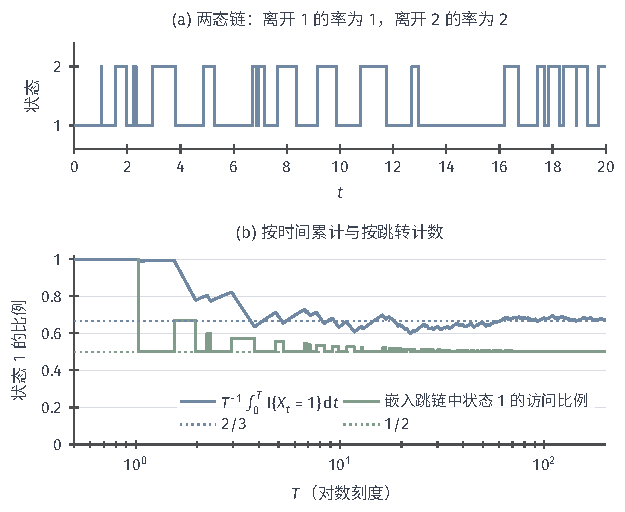
\includegraphics[width=105mm]{figures/03-optimization-evolution-and-signals/02-processes-and-trajectory-evolution/tikz/ctsp-occupation-embedded/figure.pdf}
  \caption{按时间累计与按跳转计数。两态链离开状态$1$的率为$1$，离开状态$2$的率为$2$，从状态$1$出发，固定随机种子。(a)前$20$个时间单位的路径，状态$1$的停留段平均更长；(b)同一路径上，状态$1$的占据时间比例（蓝）趋于不变分布中的$2/3$，嵌入跳链中访问状态$1$的比例（绿）趋于$1/2$，横轴为对数刻度。}
  \label{fig:ctsp-occupation-embedded}
\end{figure}

一般地，若嵌入跳链有不变分布$\bm\nu$，连续时间链的不变分布满足$\pi_i\propto\nu_i/q_i$：访问频率乘以每次访问的平均停留时间$1/q_i$。两态例中$\bm\nu=(\frac12,\frac12)$，$\bm q=(1,2)$，$\nu_i/q_i=(\frac12,\frac14)$，归一化即得$(\frac23,\frac13)$。这个关系也提示一个改进：若只想估计$\int f\,\mathrm d\pi$，可以把随机的停留时间$S_k$换成它的条件期望$1/q_{Y_k}$，估计量$\sum_kf(Y_k)/q_{Y_k}\big/\sum_k1/q_{Y_k}$消去了停留时间的随机性，这是第~\ref{chap:discrete-time-stochastic-processes}章Rao--Blackwell化的又一个实例。

\paragraph{观测方式、相关性与标准误}
实际计算中有两种累计方式。事件驱动的方式按上式精确累计，计算量与跳跃次数成正比；等间隔观察的方式只记录$X_{kh}$，用$n^{-1}\sum_kf(X_{kh})$近似，它估计的是骨架链的平均，只有在骨架链遍历时才指向$\pi$（第~\ref{sec:ctsp-time-average}节）。$h$越小，相邻观测越相关，额外的观测带来的信息越少；$h$越大，单次观测越独立，但可能错过短暂的停留。

估计误差需要长期方差。在中心极限定理成立的条件下，$\bar f_T$的标准误约为$\sigma_f/\sqrt T$，其中$\sigma_f^2=2\int_0^\infty C(s)\,\mathrm ds$是第~\ref{sec:ctsp-time-average}节的长期方差。把运行时间分成若干等长的批次，用批次平均之间的离散程度估计$\sigma_f^2$，是常用的做法；它只在批次长度远大于相关时间、并且中心极限定理适用时才可靠。遍历定理本身不提供这样的误差估计。

\subsection{以目标分布为不变分布的扩散}
\label{sec:ctsp-langevin}

\paragraph{Langevin扩散}
设目标密度$\pi(\bm x)\propto e^{-U(\bm x)}$，$U$称为势函数，只需知道到相差一个常数为止。我们希望构造一个扩散，使$\pi$是它的不变分布。直观的设计是：漂移沿$-\nabla U$把状态推向高密度区域，噪声防止它停在最低点上，二者的强度匹配到恰好保持$\pi$。这就是\term{Langevin扩散}（Langevin diffusion）
\begin{equation}
  \mathrm d\bm X_t=-\nabla U(\bm X_t)\,\mathrm dt+\sqrt2\,\mathrm d\bm W_t ,
  \label{eq:ctsp-langevin}
\end{equation}
其生成元为$\mathcal Lf=\Delta f-\nabla U^\top\nabla f$。

为什么系数是$\sqrt2$，可以由生成元的一个恒等式看出。直接展开可得$e^{-U}\mathcal Lf=\nabla\cdot(e^{-U}\nabla f)$。对$f\in C^2_c$积分，散度定理给出
\[
  \int\mathcal Lf\,\mathrm d\pi=0,\qquad
  \int g\,\mathcal Lf\,\mathrm d\pi=-\int\nabla g^\top\nabla f\,\mathrm d\pi .
\]
第一式说明$\pi$满足第~\ref{sec:ctsp-invariant}节的生成元平衡条件；第二式关于$f,g$对称，说明以$\pi$启动的过程在时间反转下规律不变，即可逆。若把噪声换成$\sigma\,\mathrm d\bm W$，平衡的密度会变成$e^{-2U/\sigma^2}$，只有$\sigma=\sqrt2$时才恰好是目标。另一种常见的写法$\mathrm d\bm Y=\frac12\nabla\log\pi(\bm Y)\,\mathrm dt+\mathrm d\bm W$描述的是同一过程放慢一半的版本：令$\bm Y_s=\bm X_{s/2}$，由Brownian尺度变换即得此式，所以两者的不变分布相同。

生成元平衡只是候选验证。要把$\pi$确认为不变分布，还需$U\in C^2$、$e^{-U}$可积，以及过程不爆炸（例如$U$在无穷远处增长，使第~\ref{sec:ctsp-sde-existence}节的Lyapunov条件成立）。唯一性与收敛需要额外的论证。噪声非退化使过程可以到达任何区域，这排除了多个不变分布；收敛速度则由下面的不等式控制。

\begin{theorem}[Poincaré不等式与方差衰减]
  \label{thm:ctsp-poincare}
  设Langevin扩散良定，$\pi$为其不变分布，并且$\pi$满足\term{Poincaré不等式}（Poincaré inequality）：存在$C_{\mathrm P}>0$，使对足够光滑的$f$，
  \[
    \operatorname{Var}_\pi(f)\leq C_{\mathrm P}\int\|\nabla f\|_2^2\,\mathrm d\pi .
  \]
  则对$\pi$平方可积的$f$，$\operatorname{Var}_\pi(P_tf)\leq e^{-2t/C_{\mathrm P}}\operatorname{Var}_\pi(f)$。
\end{theorem}

\begin{proof}
不妨设$\int f\,\mathrm d\pi=0$，则$\int P_tf\,\mathrm d\pi=0$。对足够光滑的$f$，由Kolmogorov方程与上面的对称恒等式，
\[
  \begin{aligned}
    \frac{\mathrm d}{\mathrm dt}\int(P_tf)^2\,\mathrm d\pi&=2\int P_tf\,\mathcal LP_tf\,\mathrm d\pi=-2\int\|\nabla P_tf\|_2^2\,\mathrm d\pi\\
    &\leq-\frac2{C_{\mathrm P}}\int(P_tf)^2\,\mathrm d\pi .
  \end{aligned}
\]
Grönwall不等式给出结论；一般的平方可积$f$由逼近得到，所需的定义域细节见Kallenberg的教材。
\end{proof}

定义域方面的细节可参考文献\scite{math-kallenberg2021probability}。

定理说明，从任何初值分布出发，读数$f$的条件平均以速率$1/C_{\mathrm P}$趋于其$\pi$平均。$U$强凸，即$\nabla^2U\succeq\kappa\bm I$（$\kappa>0$）时，$C_{\mathrm P}\leq1/\kappa$；多峰目标的Poincaré常数则可能很大。

\paragraph{二次势：可解的检验}
取$U(\bm x)=\frac12\bm x^\top\bm\Sigma^{-1}\bm x$，目标为$\mathcal N(\bm0,\bm\Sigma)$。式~\eqref{eq:ctsp-langevin}化为线性方程$\mathrm d\bm X=-\bm\Sigma^{-1}\bm X\,\mathrm dt+\sqrt2\,\mathrm d\bm W$，由第~\ref{sec:ctsp-linear-sde}节，稳态协方差$\bm P$解Lyapunov方程$-\bm\Sigma^{-1}\bm P-\bm P\bm\Sigma^{-1}+2\bm I=\bm0$，其解正是$\bm P=\bm\Sigma$。在$\bm\Sigma$的特征方向上，过程分解为独立的OU过程，沿特征值为$s$的方向，相关性按$e^{-t/s}$衰减。最慢的方向对应$\bm\Sigma$的最大特征值，这也是此时的Poincaré常数$C_{\mathrm P}=\lambda_{\max}(\bm\Sigma)$。

这个例子说明了混合的代价来自哪里：目标在某个方向上越宽，过程沿该方向扩散得越慢。时间平均的长期方差可以按第~\ref{sec:ctsp-time-average}节计算：沿特征值为$s$的方向，$f(\bm x)$取该方向坐标时，$\sigma_f^2=2\int_0^\infty se^{-t/s}\,\mathrm dt=2s^2$。

\paragraph{多峰与缓慢混合}
平衡等式对多峰目标同样成立，但它只保证从$\pi$出发不会离开$\pi$，不保证从别处出发能很快到达$\pi$。考虑$U(x)=2(x^2-1)^2$，目标在$x=\pm1$处有两个峰，中间$x=0$处的密度只有峰值的$e^{-2}\approx0.135$倍。过程在一个峰附近停留很久，必须依靠一串方向一致的噪声才能翻过中间的低密度区域。图~\ref{fig:ctsp-langevin-double-well}画出了一条路径和它的时间直方图：路径在两个峰之间偶尔切换，长时间运行后直方图接近目标密度，但两峰的相对权重要靠足够多次切换才能估计准确。势垒越高，切换越罕见，所需的运行时间按指数增长。

\begin{figure}[htbp]
  \centering
  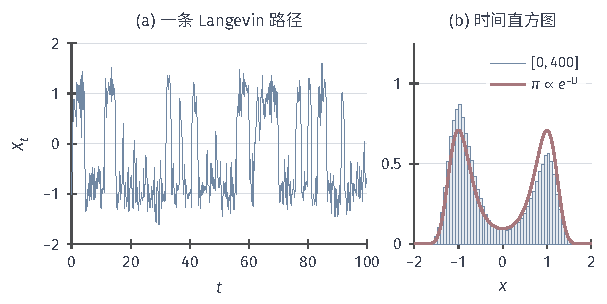
\includegraphics[width=105mm]{figures/03-optimization-evolution-and-signals/02-processes-and-trajectory-evolution/tikz/ctsp-langevin-double-well/figure.pdf}
  \caption{双峰目标上的Langevin路径。$U(x)=2(x^2-1)^2$，目标$\pi\propto e^{-U}$，用步长$2\times10^{-3}$的Euler--Maruyama离散（即下文的ULA）从$x=-1$模拟到$T=400$，固定随机种子。(a)前$100$个时间单位的路径，状态在$\pm1$附近停留并偶尔切换；(b)全部步的时间直方图与目标密度（红线）。小步长下离散偏差很小，直方图与目标的差主要来自切换次数有限。}
  \label{fig:ctsp-langevin-double-well}
\end{figure}

\subsection{连续采样的离散实现}
\label{sec:ctsp-ula-mala}

\paragraph{未校正Langevin算法}
连续扩散不能直接在计算机上运行。用Euler--Maruyama离散式~\eqref{eq:ctsp-langevin}，得到\term{未校正Langevin算法}（unadjusted Langevin algorithm，ULA）
\begin{equation}
  \bm X_{k+1}=\bm X_k-h\nabla U(\bm X_k)+\sqrt{2h}\,\bm\xi_k,\qquad\bm\xi_k\sim\mathcal N(\bm0,\bm I).
  \label{eq:ctsp-ula}
\end{equation}
每一步需要一次梯度求值和一组高斯数，不需要计算$\pi$的归一化常数。

ULA的误差有三个来源，应分别看待。第一是有限时间的路径误差，由第~\ref{sec:ctsp-error-types}节控制，在有限时段上随$h\to0$消失。第二是不变分布的偏差：数值链的长期分布不是$\pi$。第三是有限运行时间带来的初值遗留与抽样误差，由混合速度和长期方差决定。第二项不随运行时间的增加而消失。

一维标准高斯目标可以算出这个偏差。$U(x)=x^2/2$时，ULA为$X_{k+1}=(1-h)X_k+\sqrt{2h}\,\xi_k$，只有在$0<h<2$时稳定，其稳态方差为
\[
  \frac{2h}{1-(1-h)^2}=\frac1{1-h/2},
\]
而目标方差为$1$。$h=0.2$时偏高约$11\%$，$h=1$时偏高一倍。连续模型对任何初值都收敛，数值链却在$h\geq2$时发散：离散稳定性必须单独检查。对二次势$U=\frac12\bm x^\top\bm\Sigma^{-1}\bm x$，稳定要求$h<2\lambda_{\min}(\bm\Sigma)$，而最慢方向的松弛需要约$\lambda_{\max}(\bm\Sigma)/h$步；两者合起来，所需步数至少与条件数$\lambda_{\max}/\lambda_{\min}$成正比。

\paragraph{Metropolis调整的Langevin算法}
消除不变分布偏差的办法，是把ULA的一步当作提议，再用第~\ref{chap:discrete-time-stochastic-processes}章的Metropolis--Hastings规则决定是否接受。从$\bm x$出发的提议分布为
\[
  q(\bm x,\bm y)\propto\exp\Bigl\{-\frac{\|\bm y-\bm x+h\nabla U(\bm x)\|_2^2}{4h}\Bigr\},
\]
即均值$\bm x-h\nabla U(\bm x)$、协方差$2h\bm I$的高斯分布。它不对称，接受概率必须包含反向提议密度：
\begin{equation}
  \alpha(\bm x,\bm y)=\min\Bigl\{1,\frac{\pi(\bm y)\,q(\bm y,\bm x)}{\pi(\bm x)\,q(\bm x,\bm y)}\Bigr\},
  \label{eq:ctsp-mala}
\end{equation}
被拒绝时留在$\bm x$。这称为\term{Metropolis调整的Langevin算法}（Metropolis-adjusted Langevin algorithm，MALA）。由Metropolis--Hastings的细致平衡，$\pi$对任何$h>0$都是精确的不变分布。计算反向密度$q(\bm y,\bm x)$需要$\nabla U(\bm y)$，若提议被接受，这个梯度在下一步可以复用，所以每步的主要代价仍是一次梯度和一次势函数求值。

图~\ref{fig:ctsp-ula-mala}比较了两种算法。ULA的长期方差随步长偏离$1$，模拟值紧贴理论曲线$1/(1-h/2)$；MALA在所有步长下都停在$1$附近。代价体现在接受率上：步长增大时，提议越来越大胆，被拒绝得越来越多，链停在原地的时间变长，有效样本随之减少。接受校正消除的是偏差，不是相关性。

\begin{figure}[htbp]
  \centering
  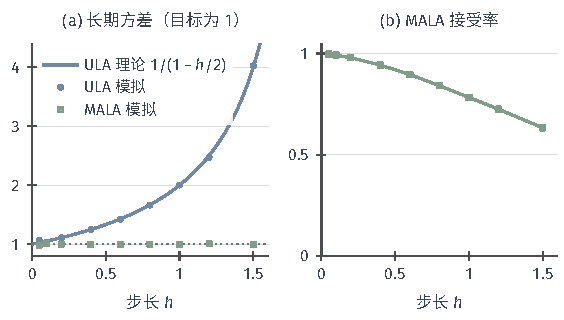
\includegraphics[width=96mm]{figures/03-optimization-evolution-and-signals/02-processes-and-trajectory-evolution/tikz/ctsp-ula-mala/figure.pdf}
  \caption{标准高斯目标上的ULA与MALA。每个步长$h$各运行$1.2\times10^5$步，从$0$出发，固定随机种子。(a)$X^2$的时间平均，即长期方差的估计：ULA（蓝点）沿理论曲线$1/(1-h/2)$偏离目标值$1$，MALA（绿点）保持在$1$附近；(b)MALA的平均接受率随步长下降。}
  \label{fig:ctsp-ula-mala}
\end{figure}

ULA与MALA本身都是离散时间的Markov链，它们的遍历性与误差分析属于第~\ref{chap:discrete-time-stochastic-processes}章的框架。把它们放在这里，是为了说明一个连续时间模型怎样变成可以执行的采样方法：连续扩散提供“往哪里走、走多远”的设计，离散化提供计算步骤，接受校正修复离散化引入的偏差。

\subsection{连续路径换测度（补充）}
\label{sec:ctsp-girsanov}

\paragraph{从有限路径的似然比出发}
第~\ref{chap:discrete-time-stochastic-processes}章的路径重加权把有限路径在两个模型下的密度之比写成各步条件密度之比的连乘。对连续时间扩散，可以先在网格上写出这个比值，再看网格加细时会发生什么。设两个模型$\mathrm dX=\beta(X)\,\mathrm dt+\mathrm dW$与$\mathrm dX=\mathrm dW$，在步长$h$的Euler离散下，一步转移密度之比为
\[
  \frac{\exp\{-(\Delta X-\beta h)^2/(2h)\}}{\exp\{-(\Delta X)^2/(2h)\}}=\exp\Bigl\{\beta\,\Delta X-\frac12\beta^2h\Bigr\}.
\]
连乘以后，指数是$\sum\beta(X_{t_k})\Delta X_k-\frac12\sum\beta(X_{t_k})^2h$，网格加细时它趋于$\int_0^T\beta\,\mathrm dX-\frac12\int_0^T\beta^2\,\mathrm dt$。分母中的$h$恰好相消，这是两个模型扩散系数相同的结果。若扩散系数不同，每一步的比值都带有一个与$h$有关的常数因子，连乘后发散或趋零，极限不存在。所以连续路径的似然比不能无条件地由离散连乘取极限得到，需要单独的定理。

\paragraph{随机指数与Novikov条件}
设$\bm\theta$是$\mathbb R^m$值的可预测过程，$\int_0^T\|\bm\theta_s\|_2^2\,\mathrm ds<\infty$几乎必然，定义
\begin{equation}
  Z_t=\exp\Bigl\{\int_0^t\bm\theta_s^\top\mathrm d\bm W_s-\frac12\int_0^t\|\bm\theta_s\|_2^2\,\mathrm ds\Bigr\},
  \label{eq:ctsp-stochastic-exponential}
\end{equation}
称为\term{随机指数}（stochastic exponential）。由Itô公式，$\mathrm dZ_t=Z_t\bm\theta_t^\top\mathrm d\bm W_t$，漂移恰好消失，所以$Z$是正的局部鞅，由第~\ref{sec:ctsp-continuous-martingales}节它是超鞅，$\mathbb EZ_T\leq1$。$Z$能否作为密度，取决于$\mathbb EZ_T=1$是否成立，即$Z$是否为真鞅。一个常用的充分条件是\term{Novikov条件}（Novikov condition）
\begin{equation}
  \mathbb E\exp\Bigl\{\frac12\int_0^T\|\bm\theta_s\|_2^2\,\mathrm ds\Bigr\}<\infty ,
  \label{eq:ctsp-novikov}
\end{equation}
其证明见Øksendal的教材\scite{math-oksendal2003sde}。若$\|\bm\theta\|_2\leq c$，被积指数不超过$c^2T/2$，条件自然成立。

\paragraph{Girsanov定理}
当$Z$是真鞅时，可以用它定义新的概率测度，并精确描述Brownian运动在新测度下的样子。换测度的一般框架，即用非负、期望为一的随机变量作为Radon--Nikodym密度定义新测度，见\BookChapterRef{chap:densities-change-of-measure}{卷二“密度与换测度”章}。

\begin{theorem}[Girsanov定理]
  \label{thm:ctsp-girsanov}
  设$Z$由式~\eqref{eq:ctsp-stochastic-exponential}定义且$\mathbb EZ_T=1$。令$\mathrm d\mathbb Q=Z_T\,\mathrm d\mathbb P$于$\mathcal F_T$。则在$\mathbb Q$下，
  \[
    \widetilde{\bm W}_t=\bm W_t-\int_0^t\bm\theta_s\,\mathrm ds,\qquad0\leq t\leq T,
  \]
  是标准Brownian运动。
\end{theorem}

定理~\ref{thm:ctsp-girsanov}称为\term{Girsanov定理}（Girsanov theorem）。它的证明需要Lévy的Brownian刻画（连续局部鞅、二次变差为$t$即为Brownian运动），这里只解释它的含义\scite{math-kallenberg2021probability}。在原测度下，$\bm W$没有漂移；换到$\mathbb Q$以后，$\bm W$获得漂移$\bm\theta$，而扣掉这一漂移的$\widetilde{\bm W}$成为新的Brownian运动。换测度只改变漂移，不改变二次变差：二次变差是沿路径加细分割得到的极限，在一个测度下几乎必然成立的事，在与之等价的测度下也几乎必然成立。

应用于扩散，设$\mathrm d\bm X=\bm b(\bm X)\,\mathrm dt+\bm\sigma\,\mathrm d\bm W$在$\mathbb P$下成立，$\bm\sigma$可逆。取$\bm\theta=\bm\sigma^{-1}(\bm b'-\bm b)(\bm X)$，则在$\mathbb Q$下$\mathrm d\bm X=\bm b'(\bm X)\,\mathrm dt+\bm\sigma\,\mathrm d\widetilde{\bm W}$。于是任何路径泛函$F$满足
\[
  \mathbb E_{\mathbb Q}F(\bm X_{[0,T]})=\mathbb E_{\mathbb P}\bigl[Z_TF(\bm X_{[0,T]})\bigr]:
\]
可以在一个模型下模拟路径，乘以权重$Z_T$，估计另一个模型下的期望。这是有限路径重加权的连续时间版本。

\begin{example}[用漂移估计罕见事件]
  \label{ex:ctsp-girsanov-rare-event}
  估计$p=\mathbb P(W_1>4)=1-\Phi(4)\approx3.17\times10^{-5}$。直接模拟时，每$31574$个样本平均只有一个落入事件，相对方差$(1-p)/p\approx3.16\times10^4$，要使相对误差降到$10\%$约需$3.2\times10^6$个样本。改在常数漂移$\theta=4$下模拟，即$W_1\sim\mathcal N(4,1)$，并乘以权重$\exp\{-4W_1+8\}$（$Z_1^{-1}$），估计量的二阶矩为$e^{16}[1-\Phi(8)]\approx5.53\times10^{-9}$，相对方差约为$4.5$，同样的精度只需约$450$个样本。漂移把路径推向罕见事件发生的区域，权重则精确地抵消了这一推动。
\end{example}

\paragraph{需要分别核对的条件}
例子中的方差缩减并不是一般规律。权重是合法密度（$\mathbb EZ_T=1$）与权重的二阶矩有限是两个不同的条件：前者保证估计量无偏，后者保证估计量的方差有限。漂移差很大或时域很长时，$Z_T$可能高度偏斜，少数路径携带几乎全部权重，这与离散长路径的权重退化是同一现象。

两个扩散系数不同的模型，其路径规律一般相互奇异，没有密度可言。以$W$与$2W$为例，在$[0,T]$上前者的二次变差为$T$，后者为$4T$；事件“二次变差等于$T$”在一个模型下概率为一，在另一个模型下概率为零。所以连续路径的换测度只能改变漂移，不能当然地改变扩散系数。基于路径权重评价行动策略属于后续的决策与控制部分，依据观测对路径重加权属于第~\ref{chap:state-space-estimation}章，这里只建立路径权重的概率关系。
